\chapter{Trees} \label{tree}

\section{Balanced Trees}

A tree is balanced when each level of the tree (except possibly the last
level) has as many nodes as it can hold. .   More formally a binary tree is balanced if, for every node in the tree,  the number of inner nodes of the left and right subtrees differs by at most 1.

Another way to define a balanced tree is to think about the depth of the  leaf nodes.   A binary tree is balanced if the difference in depth of any two leaf nodes is at most one.
The tree below is balanced
because all of the nodes have  left and right subtrees  with the same number of nodes except for
left most bottom subtree which has a node-difference of 1 between its left and right subtrees.


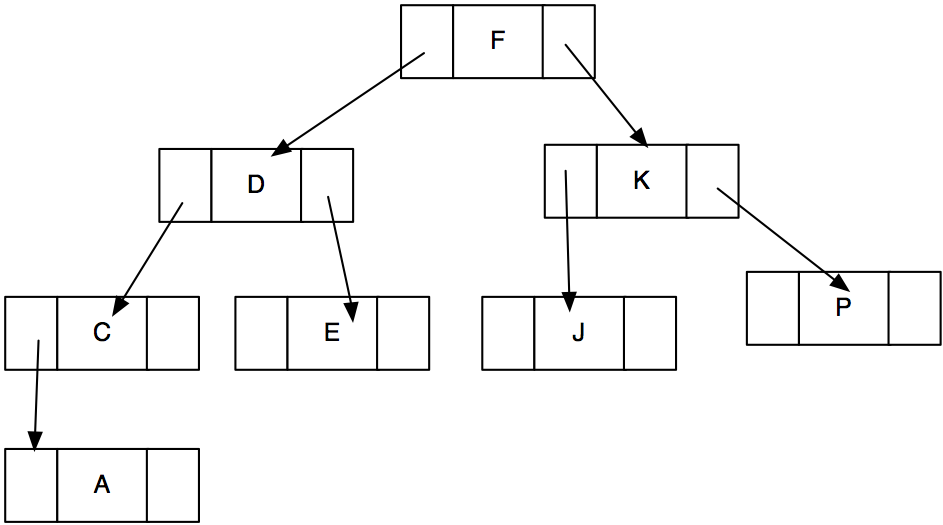
\includegraphics{pictures/image6.png}

Because sorted trees can be very sensitive to input order, they can quickly
become unbalanced.  For example,  try to sketch the binary tree that results from adding the
following nodes (in the order given): A C D E F J K P    

An unbalanced tree does not have O(log N) speed for operations and could be as poor as O(N) if the tree becomes a linked list due to input order.  It is desirable to keep binary trees balanced.

A tree can be rebalanced , but the rebalancing operation must not violate the sorting rule for the
 the nodes in the tree and it must be more efficient than
simply rebuilding the tree by randomizing the input order. The operation
used to rebalance a tree is called a \textbf{rotation}.   The exact algorithm for performing rotations depends on the type of tree.

The figure below shows an unbalanced tree of three nodes. The sort-order of the tree is that larger elements are placed in the right subtree.  The tree is unbalanced to the
right.  We can determine this because the height of the right subtree is 2 but the height of the left subtree is 0.  The right subtree is more than one higher than the left subtree.    This tree can be rebalanced by rotating  the right subtree to the right, which causes the middle node to become the new root node.   The rotation does not violate the sort-order rule for this tree, but this particular
rotation operation can only work if the middle node (the one that will
be the new root) has no left tree.

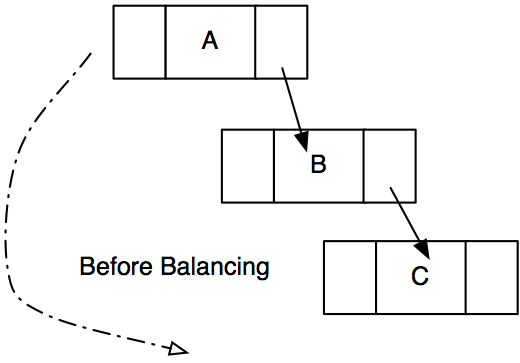
\includegraphics{pictures/image7.png}

After the rotation the tree will have B as the root node and will have two subtrees of height 1, leaving the tree in a balanced state.

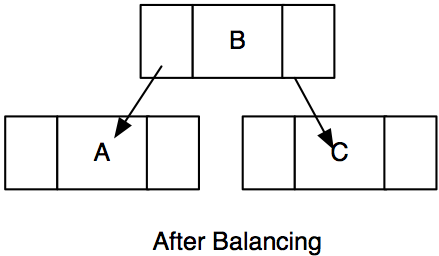
\includegraphics{pictures/image8.png}

A similar subtree tree that is unbalanced to the left can be rebalanced using a rotation to
the right.  The tree shown below is unbalanced because the left subtree has a height of two and the right subtree has a height of zero.  

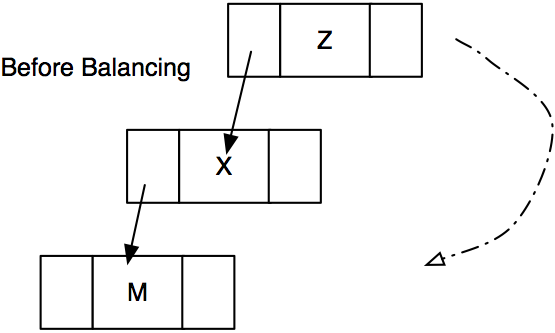
\includegraphics{pictures/image9.png}
This type of right rotation is only possible if the middle node has no
right subtree.  After the rotation, the tree looks like this:

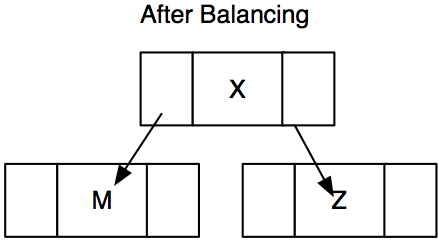
\includegraphics{pictures/image10.png}

Sequences of left and right rotations using subtrees of an unbalanced tree can be used to rebalanced the tree. In the next few sections we will explore the use of rotations to
 balance binary search trees.



\section{Binary Search Trees}

One common application for binary trees is to use them as a search tree for quickly finding stored information. Binary trees are fast, as long as they are balanced. Unfortunately, in the worst case scenario (if the data is entered sorted, for example), a binary search tree has O(N) complexity for insertion and retrieval.  (Can you explain why  this the case?)

To mitigate the problems associated with the order of insertions, specialized binary search trees have been developed that maintain the balance of the tree as data is entered and removed. There are many types of search trees including AVL trees, B trees, 2-3 trees, Red-black trees, Splay trees, and  skip lists. We will examine two such trees, AVL trees and B trees.


\subsection{AVL trees}

The AVL tree was proposed in 1962 as a solution to the problems with binary search trees. It is named in honour of the authors of the original paper introducing the tree, Adel'son-Velskii and Landis.

An AVL tree maintains the balance of the binary tree by rearranging the tree on insert and delete to carefully manage the height difference of the children of every node.

For example, in the three shown below 5 has just been inserted into the tree. The left subtree of node 82 has height of 2 and the right subtree of node 82 has height of 0. The height difference between the two subtrees of node 82 is greater than one, which indicates that the tree must be rebalanced.

\begin{figure}[H]
\centering
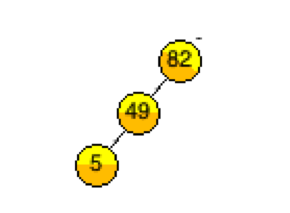
\includegraphics{pictures/tree1.png}
\caption{Unbalanced Tree}
\label{fig:tree1}
\end{figure}

A \textbf{right rotation} is performed on the \textbf{left child} of the unbalanced node, leaving a rebalanced tree. Notice that the root node of the tree has changed (it is now node 49) but the tree still meets the sorting rule for this binary tree.

\begin{figure}[H]
\centering
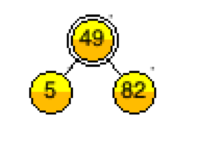
\includegraphics{pictures/tree2.png}
\caption{Rebalanced Tree}
\label{fig:tree2}
\end{figure}

Node 74 is then added to the tree. After insertion the right subtree of node 49 has a height of two and the left subtree has a height of one. The difference between the two subtrees of the root node (49) is 1,  which indicates that the tree does not need to be rebalanced.

\begin{figure}[H]
\centering
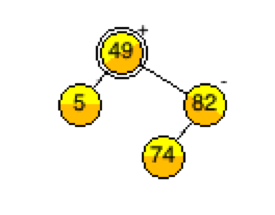
\includegraphics{pictures/tree3.png}
\caption{74 addition. Still balanced}
\label{fig:tree3}
\end{figure}

After inserting both 41 and 38 the tree is again unbalanced. While the height difference between the subtrees of node 49 is only one,  the balancing algorithm must check the height differences of all subtrees as well.  The left subtree of node 5 has a height of zero and the right subtree of node 5 has a height of two, which indicates a need to rebalance that subtree tree.

\begin{figure}[H]
\centering
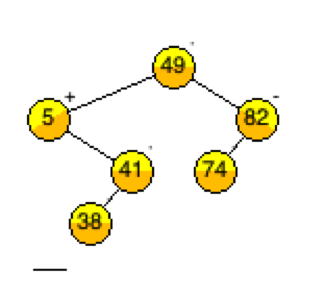
\includegraphics{pictures/tree4.png}
\caption{41 and 38 added. Tree is now unbalanced}
\label{fig:tree4}
\end{figure}

We cannot rebalance this tree with a simple rotation because the imbalance is not all with right or left children.  41 is a right child of 5 but 38 is a left child of 41.  
This tree must be rebalanced in two steps.  Intuititvely we know that we must end up with  38 as the root and make node 5 a child of node 38. 
The process is to do an initial rotation to create a subtree of all right (or all left) children, and then do the appropriate rotation on that intermediate subtree to balance.
The first step in accomplishing this is to do a right rotation with node 5's right child (41) which switches the places of nodes 38 and 41.   41 has one child (38) and no left child.  If we do a right rotation on 41,  38 becomes the root of the subtree, 41 becomes its child.

Nodes 5, 38, and 41 are now in order (and all in right subtrees), but the tree is still unbalanced.

\begin{figure}[H]
\centering
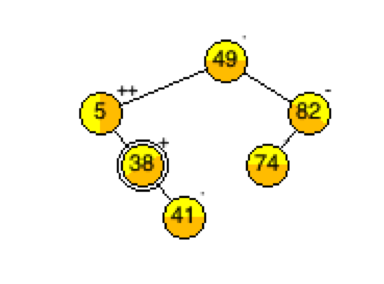
\includegraphics{pictures/tree5.png}
\caption{First rotation}
\label{fig:tree5}
\end{figure}

The second step is to do a left rotation with node 5, which rotates node 38 into the parent position.   This is the same left rotation that was illustrated at the beginning of this section.  It simply turns the middle node in the 3-node subtree into the root node, making the old root node the left child.

\begin{figure}[H]
\centering
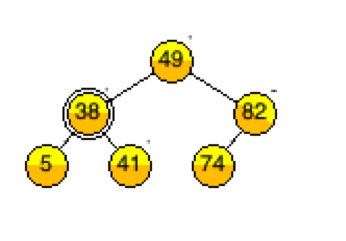
\includegraphics{pictures/tree6.png}
\caption{Second rotation}
\label{fig:tree6}
\end{figure}

After adding 21, then 25 to this tree, node 5 is unbalanced.   We must rebalance that subtree.

\begin{figure}[H]
\centering
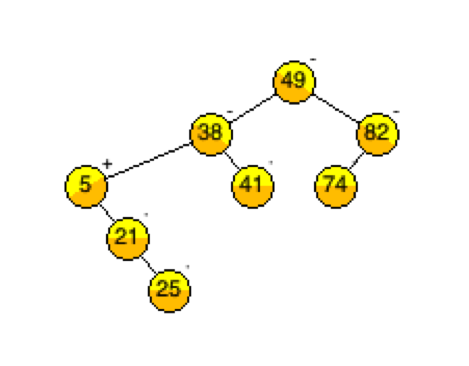
\includegraphics{pictures/tree7.png}
\caption{21 and 25 are added to the tree. Tree is now unbalanced}
\label{fig:tree7}
\end{figure}

The subtree  can be rebalanced by doing a left rotation on  the subtree.  Because the subtree is already in a straight line,  a single left rotation will rebalance it, leaving 21 as the root of the subtree with 5 and 25 as its children.

\begin{figure}[H]
\centering
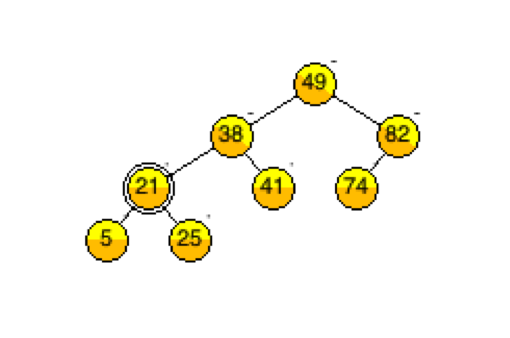
\includegraphics{pictures/tree8.png}
\caption{Left rotation on 5}
\label{fig:tree8}
\end{figure}

If 35 is added to this tree, node 21 is balanced, but node 38 is out of balance.

\begin{figure}[H]
\centering
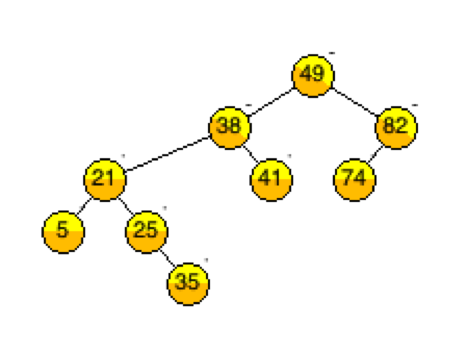
\includegraphics{pictures/tree9.png}
\caption{35 addition. Tree is now unbalanced}
\label{fig:tree9}
\end{figure}

Two rotations are required to rebalance the resulting tree. First the left subtree of node 38 must be rotated left and then the entire subtree tree rooted at 38 must be rotated right, leaving 25 as the root node of the subtree.   35 becomes the child of 38, and 38 becomes the child of 25.  There is often a need for more than one rotation to maintain balance  of an AVL tree.


\begin{figure}[H]
\centering
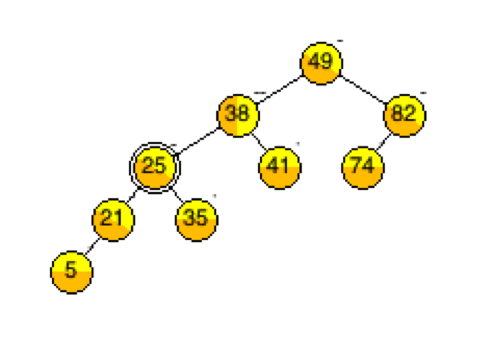
\includegraphics{pictures/tree11.png}
\caption{First rotation. Right rotation on 38 next.}
\label{fig:tree11}
\end{figure}

The same rotation rules apply when deleting nodes from the tree. While the rotations can seem complicated, the AVL tree is actually fairly simple once you understand the patterns for selecting the rotations.




\subsubsection{Nodes for AVL trees}

To facilitate the balancing of the trees, each node in an AVL tree contains an additional member that is the height of the subtree rooted at that node.   Some algorithms for AVL trees count a tree of one node as height 1 rather than height 0.     This reference material uses height 1 as the height for The height attribute of each node is used to compute whether or not the tree is balanced.

\begin{figure}[H]
\centering
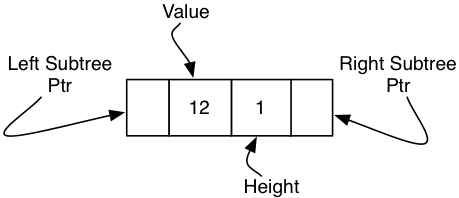
\includegraphics{pictures/tree12.png}
\caption{Tree node containing a pointer for left subtree, right subtree, an integer value and an integer height attribute}
\label{fig:tree12}
\end{figure}

A balanced AVL tree has no subtrees for which differences in height between left and right children is more than 1.

Consider the example below: The root node in the first tree has a height of 2 because it has a left child. The child has a height of 1.  The height of a node is its distance from the furthest leaf node + 1, for the purposes of the algorithms  given here for balancing an AVL tree.

\begin{figure}[H]
\centering
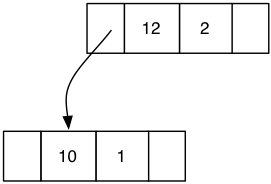
\includegraphics{pictures/tree13.png}
\caption{Tree node with 10 left child}
\label{fig:tree13}
\end{figure}

The next example shows a tree of height 3, with the heights of the children shown as well. Notice that the root node has two children, one with a height of 2 and one with a height of 1. Because the difference in heights of these two children is 1, the tree is still a balanced AVL tree.

\begin{figure}[H]
\centering
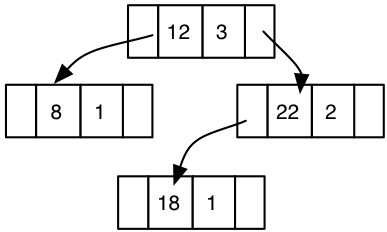
\includegraphics{pictures/tree14.png}
\caption{Balanced Tree}
\label{fig:tree14}
\end{figure}

While the examples in the picture show an AVL tree storing integers, it is far more useful to have an AVL tree that is abstracted to store any type of data. One possible design for the c structures for an AVL tree is shown below. Notice that the AVLTree is separate from the AVLTreeNodes. This permits the use of function pointers to compare and destroy the void data types without any requirement that the tree library has knowledge of what those data types are.  


\begin{lstlisting}
struct  AVLTreeNode{
    void * data;
    int nodeBalance;
    struct AVLTreeNode * left;
    struct AVLTreeNode * right;
};\end{lstlisting}


\begin{lstlisting}
struct AVLTree {
    struct AVLTreeNode * root;
    int (*compare) (void * data1, void * data2);
    void (* destroy) (void * data);
};\end{lstlisting}


\subsubsection{AVL Tree Operations}

The interface/function requirements for an AVL tree are the same as those of any binary tree. The user of the AVL tree library will need at least the following functionality.
\begin{lstlisting}
Tree * createAVLTree(int (*comparePointer) (void * data1, void * data2), void (*destroyPointer) (void *));
void  destroyAVLTree(Tree * toDie);
void addToTree(Tree * theTree, void * data);
void removeFromTree(Tree * theTree, void * data);
bool isInTree(Tree * theTree, void * data);

\end{lstlisting}

Additionally, the tree ADT will be more useful with the inclusion of pre/post and in order iterators. A simple way to implement iterator functionality is to permit only one iterator at a time on any given tree and to require a flag as a parameter to the iterator function to indicate the desired traversal. The functions required for such an iterator include a function to initialize the iterator and one to get the next value from the iterator.

\begin{lstlisting}
//Iterator functions
void  initializeIterator(Tree * theTree, int traversalType);
void * interatorNext(Tree *theTree);
\end{lstlisting}

Finally, the user of the tree ADT might appreciate some utility functions to help with writing specialized operations for the tree. These might include functions for determining if the tree is empty and functions for examining subtrees of the tree.

\begin{lstlisting}
bool isTreeEmpty(Tree * theTree);
Tree * getLeftSubtree (Tree *);
Tree * getRightSubtree (Tree *);
void * getRootData(Tree *);
\end{verbatim}

The functions listed above comprise the programming interface that a \textbf{user} of the ADT would interact with. The AVL tree needs several functions that are used only by the internal operations of the tree itself. In particular, all of the programming interface functions have a parallel internal function that operates recursively on the nodes of the tree. Those functions are joined by the functions to perform the required rotations to keep the tree balanced. In the prototypes below COMPAREPTR and DESTROYPTR are the function pointers to the compare and destroy functions.


\begin{lstlisting}
//Internal functions used by Tree ADT but not exposed to user of library
TreeNode * insert(TreeNode * root, void * data, COMPAREPTR);
TreeNode * delete(TreeNode * root, void * data,COMPAREPTR, DESTROYPTR);
TreeNode * find(TreeNode * root, void * data, COMPAREPTR);
TreeNode * findMin(TreeNode *);
TreeNode * findMax(TreeNode *);
bool isEmpty(TreeNode * root);
void destroy(TreeNode * root,DESTROYPTR);
 \end{lstlisting}
 
\subsubsection{Algorithms for Balancing AVL Trees}

Most AVL tree functions are nearly identical to the functions found in a Binary Tree ADT with the exception of the insert and delete functions. Insert and delete have an additional balancing step that is invoked to ensure that the AVL tree remains in a balanced state after each insertion and deletion. An AVL tree is said to be balanced when the height difference between left and right subtrees is either 0 or 1 for every node in the tree. 

Some AVL tree implementations keep track of the height of a node (from leaf to current node, starting counting at 1), some implementations keep track of the positive or negative balance factor for each node.  The algorithms presented here keeps track of the heights of nodes and calculates the balance factor as needed.

When a tree becomes unbalanced, there are four possible situations:
\begin{itemize}
	\item a) the imbalance occurs in right subtrees
	\item b) the imbalance occurs in left subtrees
	\item c) the imbalance occurs in a right then left subtree
	\item d) the imbalance occurs in a left then right subtree
\end{itemize}


Each of the images below shows a three node tree that matches each of the cases above. Notice that each root node has a height of 3, has a single child that is height two, which means that the difference in heights of the nodes right and left children is greater than one.

\begin{figure}[H]
\centering
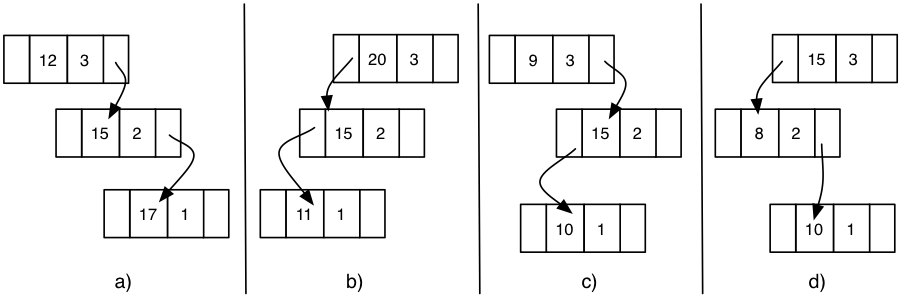
\includegraphics{pictures/tree15.png}
\caption{Unbalanced Tree Cases}
\label{fig:tree15}
\end{figure}

The solution to such imbalances is to rotate the subtree to restore balance. In all cases it is important to maintain the sorting rule for the binary tree.

These cases hold even if the tree is a larger tree in which all nodes have children. The children of the newly assigned root in rotated subtrees are reassigned to the new children, maintaining the binary tree sort.

Lets look at them case by case.\newline

\subsubsection{Case A: Imbalance to the right -$>$ Left Rotation.}

\begin{figure}[H]
\centering
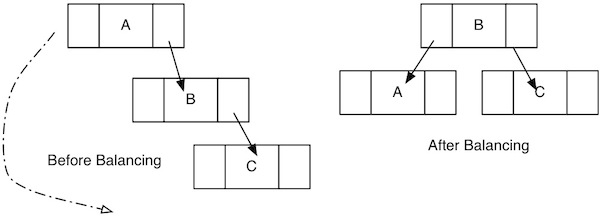
\includegraphics[width=0.5\textwidth]{pictures/leftrotate.jpg}
\caption{Left Rotation}
\label{fig:leftrotate}
\end{figure}

\begin{figure}[H]
\centering
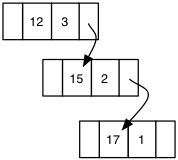
\includegraphics{pictures/tree16.png}
\caption{Right Imbalance}
\label{fig:tree16}
\end{figure}

Node 12 violates the AVL property because its right subtree has height two and its left subtree has height zero.

In this case, we know that node 12's child (15) has a value that is between node 12 and the grandchild (17). We know this because the tree is a binary tree and these are all right children.

We can make 15 the new root of this subtree, make 12 its left child, and restore balance to the tree.

This is called a \textbf{single rotation}. The resulting subtree is shown below with the heights updated. Note that 15 is now of height 2 and 12 and 17 each have height of 1.

If 15 had a left child, it would become the right child of node 12 after the rotation. This is always possible  without affecting the sorted property of the tree because node 12 initially had node 15 as the right child initially,  so all of node 15's children will have the same sort-relationship with node 12.

\begin{figure}[H]
\centering
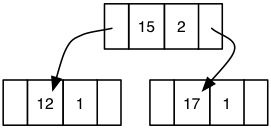
\includegraphics{pictures/tree17.png}
\caption{Balanced Tree}
\label{fig:tree17}
\end{figure}


\subsection{Case B: Imbalance to the left -$>$ Right rotation}

\begin{figure}[H]
\centering
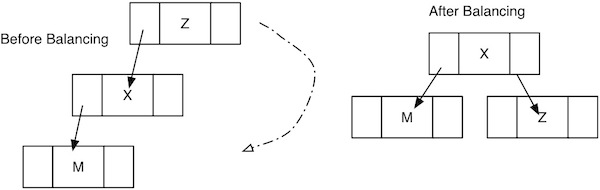
\includegraphics[width=0.5\textwidth]{pictures/rightrotate.jpg}
\caption{Right Rotation}
\label{fig:rightrotate}
\end{figure}
\begin{figure}[H]
\centering
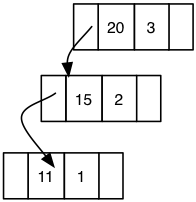
\includegraphics{pictures/tree18.png}
\caption{Left Imbalance}
\label{fig:tree18}
\end{figure}
\begin{itemize}
	\item This case is the mirror image of Case A.
	\item Node 20 is violating the AVL property. We know that its left child has a value that is ‘between’ node 20 and its grandchild.
	\item Node 15 becomes the new root, Node 20 becomes the right child and node 11 remains as the left child.
	\item This is also a single rotation (to the right).
\begin{itemize}
	\item Any right child of node 15 becomes the left child of node 20 after the rotation.
\end{itemize}
\end{itemize}

\subsection{Case C: Imbalance in left subtree of right child – double rotation}

\begin{figure}[H]
\centering
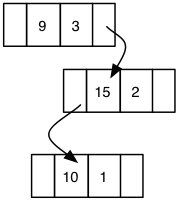
\includegraphics{pictures/tree19.png}
\caption{Imbalance in left subtree of right child}
\label{fig:tree19}
\end{figure}

\begin{itemize}
	\item In this case, a single rotation will not fix the balance problem.  The middle node (15) does not have the middle value, so we cannot simply rotate to make 15 the new root node.  
	\item Instead we perform two rotations. The first is a right rotation on the child of the imbalanced node. This rotation has the effect of turning the rotation into case A.  We make node 10 a child of node 9 and making node 15 a child of node 10, but we do not update the height values as this is an intermediate step.
\begin{itemize}
	\item Any right child of node 10 becomes the left child of node 15
\end{itemize}
	\item The second rotation is a left rotation on the imbalanced node, which will restore balance to the tree.  We update the height values in the nodes after the second rotation.
\begin{itemize}
	\item Any left child of node 10 becomes the right child of node 9
\end{itemize}
\end{itemize}

\begin{figure}[H]
\centering
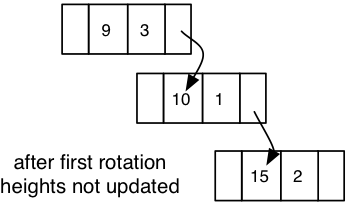
\includegraphics{pictures/tree20.png}
\caption{After first rotation. Right imbalance}
\label{fig:tree20}
\end{figure}

\begin{figure}[H]
\centering
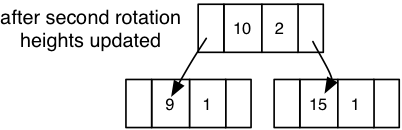
\includegraphics{pictures/tree21.png}
\caption{Balanced Tree}
\label{fig:tree21}
\end{figure}



\textbf{Case D: Imbalance due to right child of left subtree -$>$ double rotation}

\begin{figure}[H]
\centering
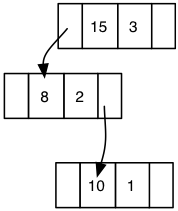
\includegraphics{pictures/tree22.png}
\caption{Imbalance in right subtree of left child}
\label{fig:tree22}
\end{figure}
\begin{itemize}
	\item This case is a mirror image of Case 3. You begin by doing a left rotation on the left child of the imbalanced node.
\begin{itemize}
	\item The left child of node 10 becomes the right child of node 8
\end{itemize}
	\item The balancing is finished by doing a right rotation on the imbalanced node.
\begin{itemize}
	\item The right child of node 10 becomes a left child of node 15
\end{itemize}
	\item In this case the result is a tree rooted at 8.
\end{itemize}



\subsubsection{AVL Tree Pseudocode}

An AVL tree ADT needs to be able to find the height of the node, it needs functions to rotateRight (with left child) and to rotateLeft (with right child). The insert function for an AVL tree can be easily written as a recursive function. An iterative function can be written to be slightly more efficient, but is much harder to write and debug (and to read).

The pseudocode is given for insert and for one set of rotation algorithms.
The remaining two rotation algorithms are mirror images of the two given and are left as an exercise. 




\begin{lstlisting}
insert(TreeNode * treeRoot, void * data): TreeNode *

  if treeRoot == NULL  create a new node with the data, return node
  else
    if the data to be inserted is less that the treeRoot data
      treeRoot->left = insert (treeRoot->left, data)  //recursive call
      //after insertion we must rebalance
      if (height of treeRoot left child is more than 1 bigger than height of treeRoot right child)
        if (data that was inserted is less than the left child)
          treeRoot = rotateRightWithLeftChild(treeRoot)  //case b
        else
          treeRoot=doubleRotateWithLeftChild(treeRoot) //case d
          
    else if the data is bigger than the treeRoot data
      treeRoot->right = insert(treeRoot->right, data) //recursive call
      //after insertion we must rebalance
      if (height of treeRoot right child is more than one taller than height of treeRoot left child)
        if (data is greater than element of right child)
          treeRoot = rotateLeftWithRightChild(treeRoot) //case a
        else
          treeRoot = doubleRotateWithRightChild(treeRoot) //case c
          
  treeRoot->height = max of child heights +1
  return treeRoot

\end{lstlisting}


Rotate right with left child is the function for the rotation noted in case b earlier in the notes.
\begin{lstlisting}
//Case B
rotateRightWithLeftChild(TreeNode * oldRoot): TreeNode *
  TreeNode * temp = oldRoot->left
  oldRoot->left = temp->right
  temp->right = oldRoot
  temp->height = max of children's heights +1
  oldRoot->height = max of children's heights +1
  return(temp)
\end{lstlisting}


\begin{lstlisting}
//case D
doubleRotateWithLeftChild (TreeNode * oldRoot): TreeNode *
  oldRoot->left = rotateWithRightChild(oldRoot->left)
  oldRoot = rotateWithLeftChild(oldRoot)
  return(oldRoot)
 	
\end{lstlisting}

Delete is somewhat more complicated for an AVL tree because of the need to maintain both the balance of the tree and the sorting-rule for the tree.   Often a lazy delete is implemented where elements are simply marked as deleted and not actually removed from the tree.  When some percentage of elements are marked as deleted a new tree is constructed from the remaining elements and the old tree is deleted.
This is an effective strategy if elements are not deleted often.

The function names given in this section are not necessarily  the same as the function names you will be asked to use for the lab portion for this section of the course.  

\clearpage
\section{B-Trees}

Suppose that you have so much data to manage that the resulting data structure cannot be held in the memory of the computer. In this case, the data structure and data must reside on persistent storage, usually some kind of drive, either attached to the computer or accessed via a network connection.  It is far more expensive in terms of time and complexity to read/write information on a disk than it is from computer memory. This  dramatically changes the cost of  operations that must traverse the search tree.  One disk access takes at least 100 000 times longer than a single operation in memory, so an ADT that stores data persistently must be designed to minimize the number of disk accesses.  

Even with a perfectly balanced AVL tree, the number of disk accesses to access information will be O(log n).  Suppose the data set in question has one million entries, log\textsubscript{2} of one million is approximately 20. If we guess that a hard drive has a seek time of 15 milliseconds, the optimistic time for a disk-based AVL tree is about 1/3 of a second per operation. That is far too slow for any type of modern data management system.

\textbf{B-Trees} are an ADT that generalize the binary tree to allow more than two branches per node.  The B-Tree is designed to reduce the number of disk accesses to a small constant number. The algorithms for operations are a bit more complicated than for other trees, but the result is a search tree that minimizes disk accesses.

B-Trees are based on the idea of adding more branches to the tree, creating an m-ary search tree rather than a binary search tree.

\begin{figure}[H]
\centering
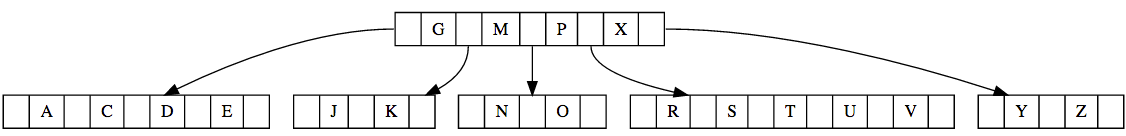
\includegraphics[width=\textwidth]{pictures/btree1.png}
\caption{B-Tree}
\label{fig:tree23}
\end{figure}

The image above shows a small b-tree with a single root node and five children. The nodes in a b-tree hold multiple data values (called keys) and have one more child node than data.   For example, the root node of the example shown above has 4 keys (data elements) and 5 children. The second child has 2 data elements and three child pointers, all currently empty.    Notice how each node in the b-tree holds more than one value.   The data element in a b-tree is called a\textbf{key}.   As with other binary trees, the data element must have a compare function that allows the elements to be ordered.

The \textbf{degree} of a b-tree defines the minimum and maximum numbers of keys and subtrees that any not can have.    The example b-tree shown has a degree of 3.   Given the degree of a tree (lets call the degree 't'),  we can state the following characteristics of the b-tree:
\begin{itemize}
\item Every node in the tree, with the exception of the root node,  must contain at least t-1 keys.   You can see in the example tree that none of the nodes contain fewer than 2 keys.
\item No node (including the root node) may contain more than 2t-1 keys.   The example tree has no nodes with 5 keys, but the number of keys in a node changes when nodes are inserted and deleted.  When the maximum number of keys is exceded, the tree must be rebalanced.
\item The number of children in a node is equal to the number of keys +1.  A node with two keys has 3 children.  A node with 4 keys has 5 children.
\item Keys are sorted in increasing order within a node.   The child tree between two nodes contains all the keys that fall between the values of the two parent keys.   The values in a child node are always less than or equal to the parent key to the right of the child and are always more than the value of the parent key to the left of the child.
\item The height of a b-tree is approximately log\textsubscript{m}N where m is the maximum number of children that a node can have (2t).
\end{itemize}


The size of the nodes is managed by splitting and combining nodes during insert and delete operations.   The figure below shows the example B-tree after adding W as a key to the tree.  

\begin{figure}[H]
\centering
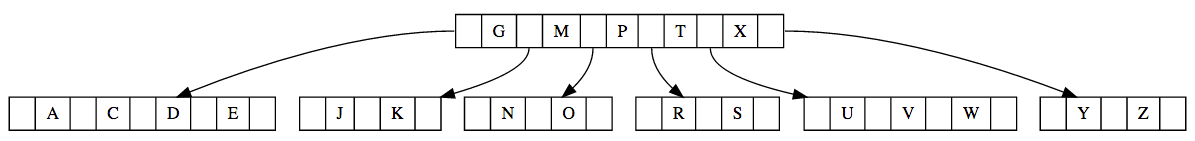
\includegraphics[width=\textwidth]{pictures/btree2.png}
\caption{Balanced B-Tree after adding W}
\label{fig:tree24}
\end{figure}

By inserting W into the tree the node containing R,S,T and U becomes too large and must be split.  The middle value (T) is  moved to the parent node and the remaining keys are split into two nodes,  R and S on the left side of T and U,V, W on the right side of T.    

All the leaf nodes of a B-tree are at the same height.  The tree is rebalanced after insertions and deletions to ensure that all leaf nodes are at the same height.    Our example B-tree is rebalanced to be of height 3 when after both B and F are added.  The addition of B and F makes the left-most child too long and it must be split.  That split increases the height of the leaf notes to 3, which necessitates rebalancing the entire tree to be of height 3.

\begin{figure}[H]
\centering
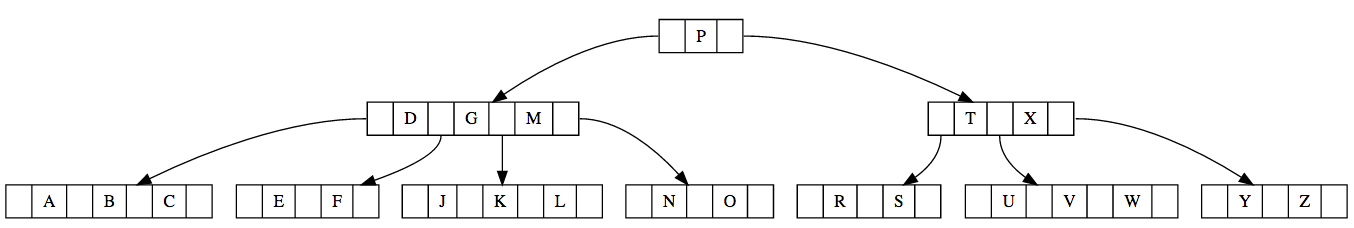
\includegraphics[width=\textwidth]{pictures/btree3.png}
\caption{Btree after the addition of B and F}
\label{fig:btree3}
\end{figure}


If a key is deleted from a node, leaving too few children in the node, a key is removed from a sibling to add to the too-empty node. This process often involves adding a new key to the parent, and moving a key from the parent into the too-empty child. Below is a figure showing the effect of removing key N from the tree shown above.   Because the removal of N leaves its node too empty, L is moved to the parent node from a sibling node, and O is  move to the child node which balances the tree and ensures that all nodes have the correct size. 

\begin{figure}[H]
\centering
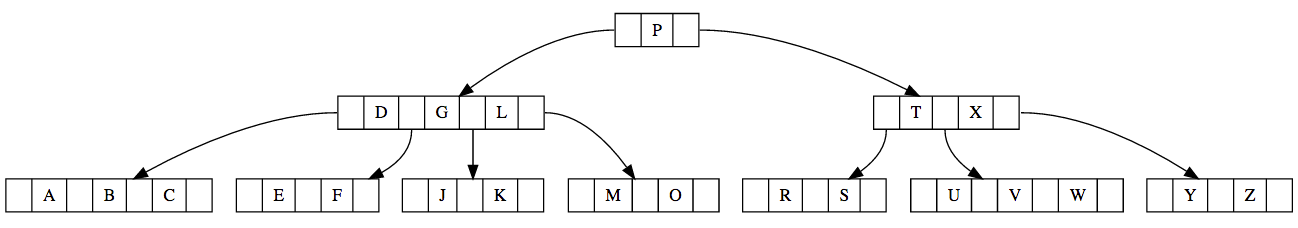
\includegraphics[width=\textwidth]{pictures/btree4.png}
\caption{Btree after removing N}
\label{fig:btree4}
\end{figure}


The algorithms for insertion and removal into b-trees are straightforward but there are many cases required to accommodate resizing the nodes. The cases for insertion and deletion can be summarized as follows:
\begin{itemize}
	\item Inserting a key into a node within the min/max parameters
\begin{itemize}
	\item Key is simply inserted
\end{itemize}
	\item Inserting a key into a node that is full
\begin{itemize}
	\item Node is split into three (two children and a root)
	\item The root is given to the parent node
\begin{itemize}
	\item May result in the parent node being split and keys being moved from it
\end{itemize}
\end{itemize}
	\item Deleting a key from a leaf node that has at least 2 more than minimum
\begin{itemize}
	\item Key is simply deleted
\end{itemize}
	\item Deleting a key from a leaf node that has only 1 more than minimum
\begin{itemize}
	\item Key is deleted
	\item If a sibling node has an extra key, a rotation is done to move the extra key to the parent and a parent’s key to the underfull child
	\item If a sibling node does not have an extra key, nodes must be deleted and recombined
\end{itemize}
	\item Deleting a key from an internal node
\begin{itemize}
	\item Rotations must be performed to ensure that the keys in the internal node are greater than or equal to the keys in the appropriate subtree.
\end{itemize}
\end{itemize}


\section{Summary}

After working through these materials you should be able to implement an AVL tree using a lazy delete strategy.  With a little bit of thinking you should be able to identify an algorithm for a direct delete for an AVL tree.  You should understand what a binary search tree is, and you should easily be able to read and understand any online resource about the other types of binary search trees.  

At this point in the course you should also be able to identify good online resources and use them to teach yourself about any data structure.  



\section{Additional Resources}
\begin{itemize}
	\item \url{http://ysangkok.github.io/js-clrs-btree/btree.html}
	\item \url{http://www.csanimated.com/animation.php?t=B-tree}
	\item \url{http://www.csanimated.com/animation.php?t=Self-balancing\_binary\_search\_tree}
	\item \url{http://www.bluerwhite.org/btree/}
\end{itemize}

\section{Extending Activities}

\begin{itemize}
\item {Using the applet found at:\url{https://people.ksp.sk/\~kuko/gnarley-trees/}, create a binary search tree (BST) by inserting the numbers between 1 and 9 into the tree, in order. What do you notice about the tree? (unclick the pause button once you understand what the insertion is doing)

Clear the tree and insert the same numbers in the following order 5 3 7 4 2 8 6 9 1 . What do you notice about the tree this time?}

\item {The tree shown in this figure is unbalanced.

  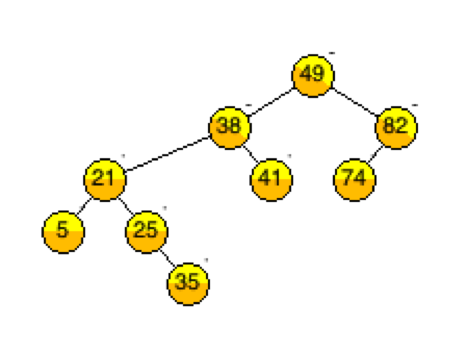
\includegraphics{pictures/tree9.png}

It needs a right rotation on node 38 to complete the balancing step.  List the steps required to complete the rotation.}

\item{ Write  C code showing the struct you would implement for a fully abstracted btree.  Write the c code for the insert function for the b-tree. }

\item{Investigate red-black trees to determine the key similarities and differences between red-black trees and AVL trees}

\item{What is the maximum height of an AVL tree with 9 nodes?  A tree with one node is height 1.   Can you find a formula for the maximum height of an AVL tree with N nodes? }

\item{Design an augmented AVL tree which can quickly compute the number of nodes in any tree or subtree.  Discuss changes to the struct for the AVL tree as well as necessary changes to any of the algorithms for the ADT.}

\end{itemize}
